\section{Návrh uživatelského rozhraní}
\label{sc:wireframes}
Návrh uživatelského rozhraní je důležitá součást vývoje software, protože to je ta část, kterou vidí uživatel. Sebelepší funkcionalita je aplikaci k~ničemu, když bude nepřehledná a příliš komplikovaná. Je několik možností, jak přistoupit k~takovému návrhu, dělené podle úrovně detailu, kterým se zabývají.

Nejvíce abstraktní, resp. nejméně se zabývající detaily je wireframe. Wireframe ukazuje část aplikace, její rozvržení a zabývá se pouze důležitými částmi. Další úrovní je mockup, který se na rozdíl od wireframu věnuje i méně podstatným částem aplikace a detailům jako jsou třeba barevná schémata či typografie. Poslední, nejpokročilejší a zároveň nejkomplikovanější možností je prototyp. Prototyp rozšiřuje mockup o~interakce, popř. animace. Umožňuje simulovat interakce mezi částmi aplikace a reprezentuje podobu konečného produktu. Rozdíl mezi prototypem a konečným produktem je, že prototyp má většinou nasimulovaná data, která by aplikace jinak získávala z~backendu. Prototypy jsou většinou vytvářeny před vývojem samotné aplikace pro zjištění, zdali má vůbec smysl takovou aplikaci vytvářet. Pokud má vývojář či tým zadaný požadavek na nějakou aplikaci, nemá smysl ztrácet čas s~prototypem, jelikož aplikaci musí dodat.

Práce uvažuje o~návrhu uživatelského rozhraní jako o~wireframu, jelikož v~kontextu této práce nemá smysl dělat prototyp. Co se týče výběru wireframu oproti mockupu, pak to je čistě subjektivní. V~praxi u~větších firem vyvíjející jednu z~mnoha aplikací je upřednostňován wireframe, jelikož detaily jako barevné schéma, či typografie se odvíjí od dalších aplikací a firemních politik. Wireframy jsou v~rozlišení $1920 \times 1080$ pixelů, tedy FullHD a byly vytvořeny v~nástroji \emph{figma.com}~\cite{figmainc_2019_figma}, který umožňuje vytváření wireframů, mockupů i prototypů.

\subsection{Stránka s~písní}
\label{ss:wireframe_song}
Nejdůležitější stránka celé aplikace. Jedná se o~komponentu z~\hyperref[uc04]{PU04}, tedy výuka písní a obsahuje komponenty~\hyperref[uc01]{Metronom},~\hyperref[uc02]{Akordy} a~\hyperref[uc03]{Strumming pattern}. Stránka obsahuje hlavní panel s~možností vyhledávání a tlačítka pro registraci a přihlášení. V~hlavní části je nejprve název písně, pak název autora a následně text a akordy písně. Zmíněné komponenty jsou po pravé straně, jelikož kdyby byly pozicovány nalevo, tak by se uživateli mohl číst špatně text, který by byl zarovnán vedle komponent. Celý obsah je na velké obrazovce odsazen na střed, tak aby se uživatel mohl soustředit pouze na část obrazovky.

\begin{figure}
    \centering
    \begin{subfigure}{\textwidth}
        \centering
        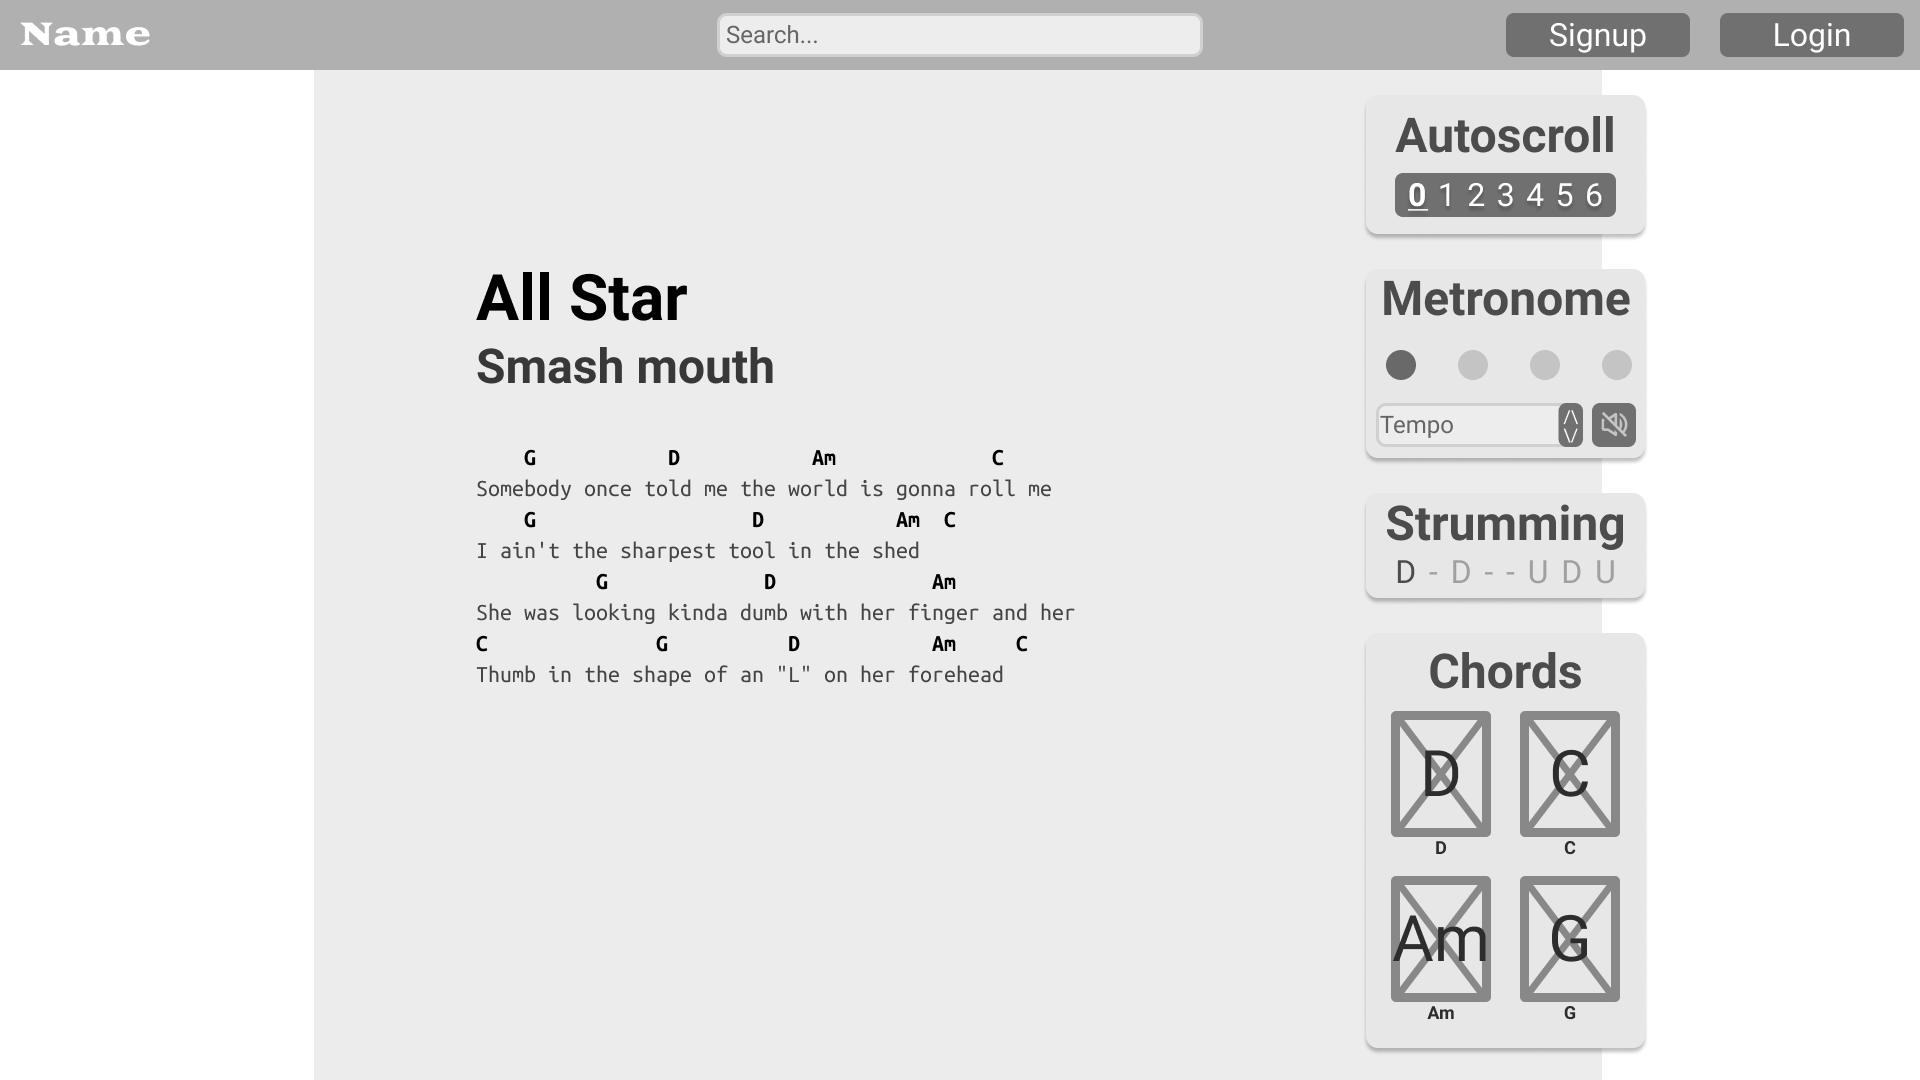
\includegraphics[width=\textwidth]{assets/song_page.png}
        \caption{Stránka s~písní}
        \label{fig:song_page}
    \end{subfigure}
    \par\bigskip
    \begin{subfigure}{.49\textwidth}
        \centering
        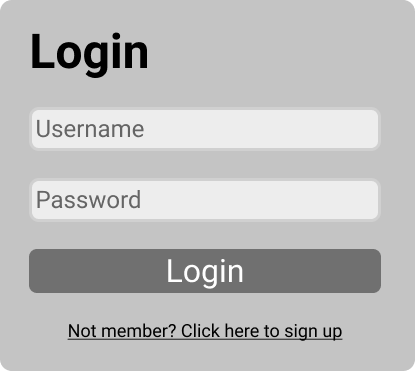
\includegraphics[width=.7\textwidth]{assets/login.png}
        \caption{Přilašovací okno}
        \label{fig:login_modal}
    \end{subfigure}
    \begin{subfigure}{.49\textwidth}
        \centering
        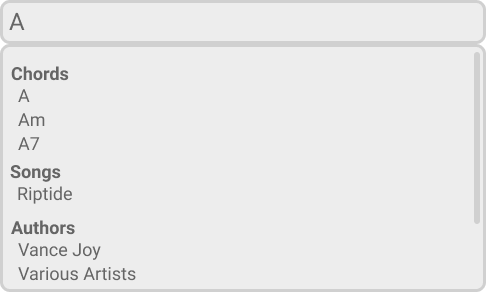
\includegraphics[width=.9\textwidth]{assets/search.png}
        \caption{Vyhledávací našeptávač}
        \label{fig:search}
    \end{subfigure}
    \caption{Wireframy}
    \label{fig:wireframes}
\end{figure}

% \begin{figure}
%     \begin{subfigure}{\textwidth}
%         \centering
%         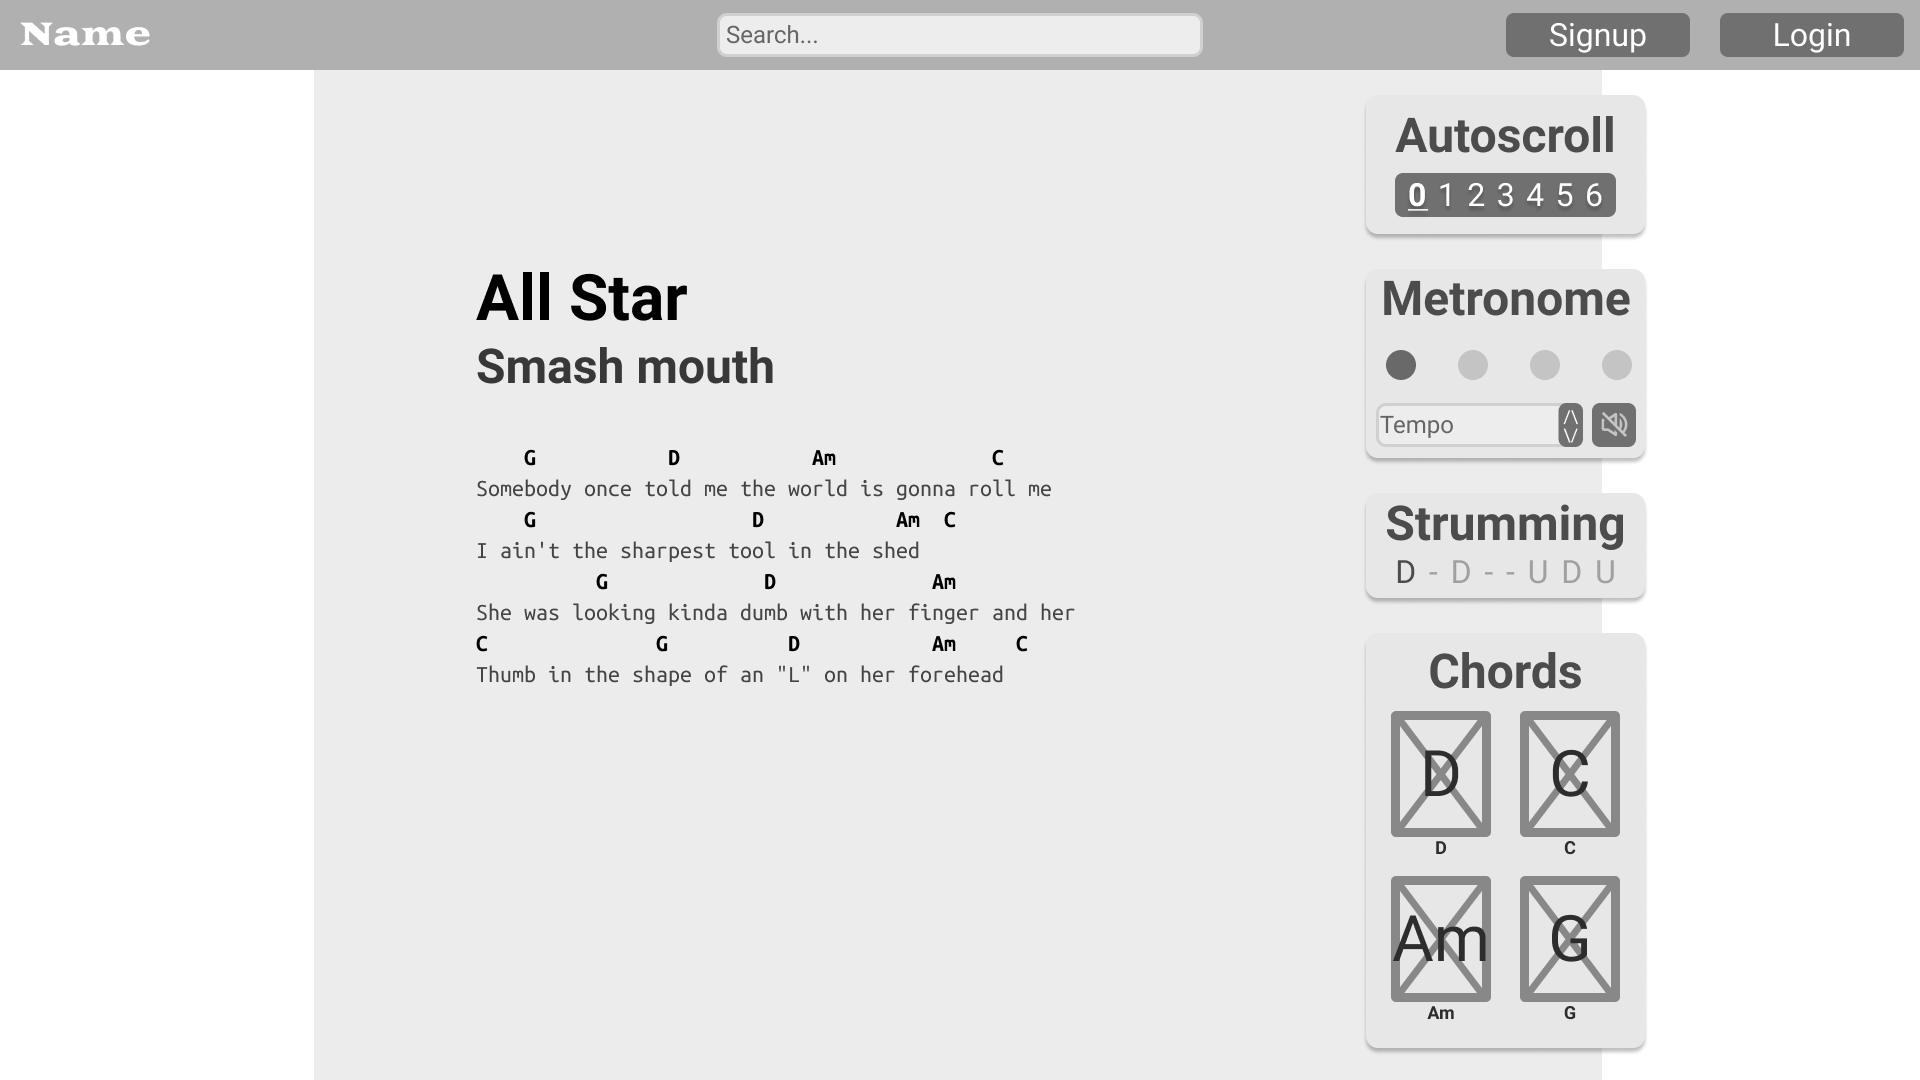
\includegraphics[width=\textwidth]{assets/song_page.png}
% \caption{Stránka s~písní}
% \label{fig:song_page}
%     \end{subfigure}

%     \medskip
%     \begin{subfigure}{.3\textwidth}
%         \centering
%         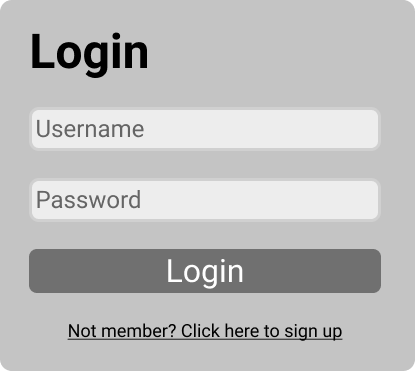
\includegraphics[width=.95\textwidth]{assets/login.png}
% \caption{Přilašovací okno}
% \label{fig:login_modal}
%     \end{subfigure}

%     \begin{subfigure}{.3\textwidth}
%         \centering
%         \includegraphics[width=.95\textwidth]{assets/signup.png}
%         \caption{Registrační okno}
%         \label{fig:signup_modal}
%     \end{subfigure}

%     \begin{subfigure}{.3\textwidth}
%         \centering
%         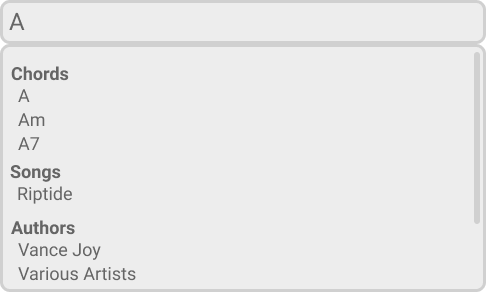
\includegraphics[width=.95\textwidth]{assets/search.png}
% \caption{Vyhledávací našeptávač}
% \label{fig:search}
%     \end{subfigure}


%     \caption{Wireframy}
%     \label{fig:wireframes}
% \end{figure}
